%Part1
\begin{concluPart}
Notre premier besoin a été de définir les types de robots qui existent, mais aussi les droits légaux d'utilisation et de dérivation de tels dispositifs. 
Ainsi, une fois passée en revue les différentes caractéristiques générales de forme et de mobilité, nous avons vu plus spécifiquement plusieurs exemples de robots pédagogiques \tiret{et leur fondement historique} qui sont aujourd'hui proposés au grand public; ainsi que leurs modalités de programmation qui passent par des langages dits visuels, des langages textuels ou des artefacts tangibles.
Mais, ces kits à visée pédagogique évoluent dans un environnement qui n'est pas neutre, il a donc été nécessaire d'étudier les conditions spécifiques de ce lieu, ainsi que les différents acteurs qui le composent. Parmi ceux-ci, élèves et enseignants \tiret{utilisateurs cible de ces dispositifs} sont des acteurs en forte interaction et celle-ci est étudiée depuis longue date.
Plusieurs approches de la pédagogie ont été ici présentées et plusieurs faits ont également été rappelés
Mais avant de s'interroger sur les leviers accessibles pour maximiser la motivation chez les jeunes, il est bon de commencer par définir la motivation.\par%
Différents points de vue s'affrontent ou se complètent. Ici, nous avons principalement abordé la vision institutionnelle et la vision issue de la meta-théorie de l'autodétermination (qui met en jeu les notions de motivation intrinsèque et extrinsèque). À cela, nous avons complété par plusieurs éléments issus des sciences cognitives nous permettant de mieux identifier certains points d'intérêt semblant \tiret{de prime abord} non déterminants.\par%
Pour mieux appréhender notre contexte  nous nous sommes également renseignés sur différents exemples du passé pour en tirer leçon; et nous constatons que le principal levier de motivation pour l'élève, au sein de l'environnement scolaire, se trouve être l'enseignant.
\citeAtion{alvarez}
Pour arriver à ses fins, il a à sa disposition un bagage de connaissances issues de sa formation dans sa discipline mais également des connaissances issues de sa formation pédagogique. C'est ce qui lui permet de générer ses propres ressources, adaptées à ses compétences et aux particularités de sa classe, pour répondre aux exigences du programme.
Notamment il sélectionne et met en scène les différentes ressources qu'il juge utile à cela.
Mais dans le contexte d'un \cro{monde numérique}: où un grand nombre de ressources sont directement accessibles en ligne et gratuitement par l'élève; l'enseignant doit adapter sa posture aux contraintes et avantages offerts par cet état de fait.\par%
Dans le contexte plus resserré de la robotique, 2~caractéristiques semblent particulièrement bénéfiques pédagogiquement: le caractère tangible des robots et le rapport à l'erreur particulier qu'implique sa programmation.\par%
Mais outre les connaissances pratiques et théoriques que possède un enseignant (de par sa formation initiale et son expérience) pour exploiter ces ressources et les adapter à sa pratique; quelles sont les connaissances spécifiques à l'informatique et la robotique qui doivent être transmises par celles-ci? 
Beaucoup des concepts élémentaires de l'informatique sont empruntés à d'autres disciplines et cela s'explique par la construction historique et épistémologique de cette discipline à l'intervalle de nombreuses autres. Cependant, elle constitue bien une discipline à part entière avec ses propres théories et ses propres paradigmes, dont plusieurs ont été présentés ici.
Concernant la robotique, nous constatons qu'un des éléments fondateur de celle-ci concerne les boucles de rétroaction permettant un contrôle plus fin des systèmes. Plus spécifiquement, nous nous restreignons, ici, aux boucles sensori-motrices mises en place par les robots pour évoluer dans leur environnement.\par%
Une fois établies, quelles connaissances transmettre et par quel vecteur, nous pouvons nous interroger sur la constitution de ces nouvelles ressources basées sur des outils interactifs. Pour cela nous pouvons nous inspirer des différents travaux déjà réalisés dans le numérique qui proposent un certain nombre de \textit{guideline}\footnote{Anglicisme pour \cro{ligne directrice}: informations destinées à informer les gens sur la manière de faire ou de pas faire quelque chose} nous aiguillant sur les éléments à sélectionner ou, au contraire, à bannir afin d'offrir la meilleure utilisabilité possible des ressources manipulées, préambule à toute construction de connaissances et de motivation.\par%
L'enseignement des sciences du numérique en France est récent. Cependant, dans quelques années, les élèves auront acquis des connaissances depuis la maternelle. On peut supposer alors que les élèves de lycée auront un niveau plus élevé. 
Il y a également une hétérogénéité de niveau des élèves d'une même classe, qui risque de s'amplifier au fur et à mesure que le niveau de difficulté augmentera. Pour anticiper ces changements, et éviter de devoir utiliser un robot spécifique par niveau, l'outil proposé devra s'adapter aux besoins et ne pas viser une utilisation trop particulière.\par%
Il devra avoir suffisamment de fonctionnalités pour permettre de générer des usages pertinents, sans être trop complexes, pour permettre à tous de l'exploiter suivant ses besoins et contraintes.
De plus, ça ne peut pas être un simple outil de démonstration, avec une boîte noire au niveau du fonctionnement ne permettant que les usages prescrits.\par%
\begin{figure}[!h]
\myDefautStyle
Ainsi, un kit robotique pédagogique destiné aux enseignants et leurs élèves en classe, se compose de différents éléments:\par%
\begin{minipage}{.38\linewidth}
  \centering
  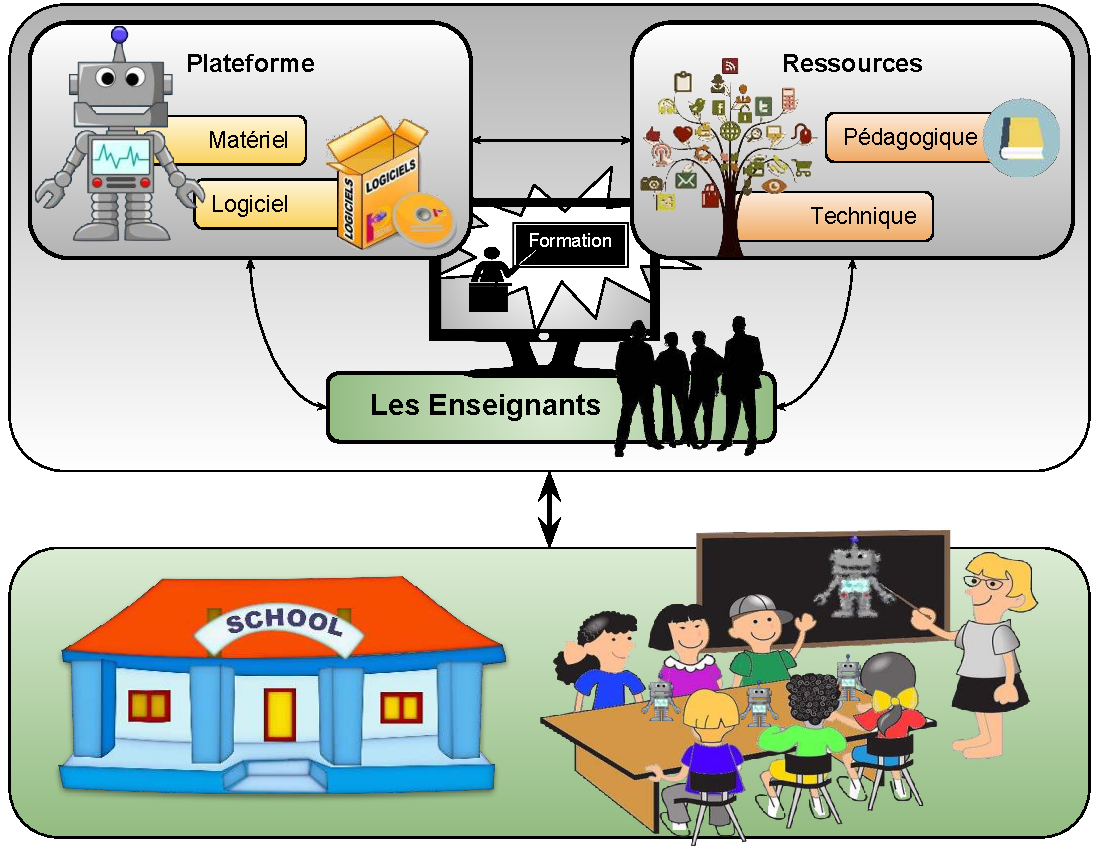
\includegraphics[width=\linewidth]{Figures/Poppy-Kit.pdf}
  \caption{Kit robotique pédagogique, Desprez~\cite{desprezPoster-efran}}\label{fig:poppy_kit}
\end{minipage}
\hfill
\begin{minipage}{.55\linewidth}
\myDefautStyle
\begin{itemize}\myItemStyle
  \item Le kit robotique en lui-même \cro{la plateforme}, comprenant le hardware et le software, ici, le robot ErgoJr contrôlé par la bibliothèque \textit{PyPot} et les langages de programmation \sht{snap} et \sht{ipy}, embarqués dans une Raspberry~Pi.
  \item Les ressources techniques (code source, documentations, entre-aide via le forum \etc) et pédagogiques (livret \citeB{noirpoudre2016livret}, activités clé en main ou dérivées) disponibles sur plusieurs supports (numérique, papier, en ligne, dans le robot, \etc)
  \item Des vecteurs de pédagogie: les enseignants aux multiples profils avec de multiples compétences ayant suivi un parcours de formation.
\end{itemize}
\end{minipage}
\end{figure}\par%
Dans une deuxième partie, nous allons voir comment s'est construit le kit pédagogique ErgoJr,ses différentes caractéristiques et les ressources qui lui sont associées. Nous présenterons également des exemples de dérivation de ce kit qui ont été réalisées.
\end{concluPart}